\documentclass[11pt,a4paper]{article}
\usepackage[utf8]{inputenc}
\usepackage[british]{babel}
\usepackage[a4paper,margin=2.3cm]{geometry}
\usepackage{amsmath,amssymb}
\usepackage{graphicx}
\usepackage{tikz}
\usetikzlibrary{calc,angles,quotes,patterns}
\usepackage[most]{tcolorbox}
\usepackage{enumitem}
\usepackage{array}
\usepackage{titlesec}
\usepackage[hidelinks]{hyperref}

\definecolor{bandgreen}{RGB}{46,139,87}
\definecolor{bandblue}{RGB}{30,100,190}
\definecolor{bandamber}{RGB}{220,140,20}
\definecolor{bandpink}{RGB}{210,70,140}
\definecolor{bandpurple}{RGB}{110,50,160}

\newcounter{prob}
% \prob{label}{title}{source}
\newcommand{\prob}[3]{\par\bigskip\refstepcounter{prob}\label{#1}%
  \noindent\textbf{\theprob.\ #2}\hfill{\small\textit{#3}}\par\nopagebreak\smallskip}
\newcommand{\ans}[2]{\par\smallskip\noindent\textbf{\ref{#1}.}\ #2}

\newcommand{\band}[3]{%
  \clearpage
  \begin{tcolorbox}[colback=#1!12,colframe=#1,boxrule=1pt,arc=2pt]
  {\Large\bfseries\color{#1} #2}\hfill{\large #3}
  \end{tcolorbox}}

\newtcolorbox{diarynote}[1]{colback=black!4,colframe=black!45,boxrule=0.6pt,
  arc=2pt,fonttitle=\bfseries\small,title={#1},fontupper=\small}

\setlength{\parindent}{0pt}
\setlength{\parskip}{3pt}
\begin{document}

\begin{titlepage}
\centering
\vspace*{3cm}
{\Huge\bfseries The Ladies' Diary\par}
\vspace{0.4cm}
{\LARGE Second book\par}
\vspace{0.8cm}
{\Large Fifty-seven problems, 1802--1816,\\ for readers from five to seventeen\par}
\vspace{2cm}
{\large\itshape Three lovely sisters uncle left\\ To them a piece of gold.\par}
\vspace{0.3cm}
{\small Question 1164, set for 1807\par}
\vfill
{\large Working draft\par}
\end{titlepage}

\section*{A word before the problems}

By 1802 the Diary was a hundred years old. Its readers still sent their answers by post
and still signed them. Some signed with a town: Mr Wm.~Burdon of Acaster Malbis,
Mr John Collins of Hatton Garden. Some signed with a joke or a mask. One signed himself
\textit{Leonardus Pisanus}, the Latin name of Fibonacci, and set a problem Fibonacci
would have recognised. The women had not gone away. Miss Mary Weston of Gainsborough,
Miss Susannah Jackson of Mile End and Mrs Elizabeth Bryhon of Helmsley all have answers
in these pages.\footnote{Leybourn, \textit{Mathematical Questions}, vol.~IV (London,
1817), answers to questions 1157, 1210, 1231, 1254 and others. The running heads of
the volume name the editor of these years as Charles Hutton.}

The problems had grown harder too. The young Olinthus Gregory and Peter Barlow, both
later of the Royal Military Academy at Woolwich, answer here as young men from Cambridge and
Shipdham. Half the volume is pendulums, water, sunlight and falling stones. Those have
been left out. What remains is pure mathematics.

Only one question in these years carries a woman's name. In 1802 Mrs Macdonald of
Spindlestone asked how large a ball of cork must be to fall through air at a steady ten
feet a second.\footnote{Question 1098. Leybourn's index lists her, wrongly, as
`Macdonal, J.'} It is physics, so it is not here. A century earlier women set the
questions as well as answering them. By 1802, in the printed record, they answered.

This booklet takes fifty-seven problems from the fourth volume of Thomas Leybourn's
collection of 1817, which gathers the Diary's questions from 1802 to 1816 with their
original answers. It is a companion to the first book, which drew on the years
1707--1748.

\subsection*{How to read the labels}

\textit{Q1231} means question~1231 in Leybourn's volume~IV, in modern words.
\textit{After Q1231} means the problem has been retold, with new numbers for younger
readers, or metres in place of feet and inches. The idea is always the Diary's. Where a
retelling changes the answer, the answer given is for the retelling. One problem keeps
its pounds and shillings, because without them it does not work.

\subsection*{The bands}

\begin{center}
\begin{tabular}{>{\bfseries}l l l r}
\color{bandgreen}Green  & ages 5--8   & folding, sharing, taking turns       & 4\\
\color{bandblue}Blue    & ages 8--11  & squares and cubes                    & 4\\
\color{bandamber}Amber  & ages 11--14 & Pythagoras, angles, first algebra    & 11\\
\color{bandpink}Pink    & ages 14--16 & GCSE: probability, trigonometry, volume & 18\\
\color{bandpurple}Purple & ages 16--17 & A-level: calculus, series, proof    & 20\\
\end{tabular}
\end{center}

Answers are at the back. When the Diary or its readers went wrong, a small grey box
says so.

\subsection*{How this edition was made}
This edition was prepared with the assistance of Claude, an AI model made by Anthropic. Under the editor's direction, Claude drafted the retellings, solutions, notes and introduction, recomputed every answer, worked from the Internet Archive's machine-read text of the source, and typeset the text. Selection, editorial decisions and final responsibility for the text are the editor's.

%================ GREEN ================
\band{bandgreen}{Green}{ages 5--8}

\prob{g1}{Four from one}{after Q1239, by Joseph Hine}
Cut a triangle out of paper. Now cut it into four smaller triangles that are all exactly
the same size and shape. \textit{Hint: find the middle of each side.}

\prob{g2}{Four fair fields}{after the prize question for 1815, by Llerien}
Four brothers share a rectangle of land. Take a rectangle of paper and fold it into four
pieces that are all the same size. Can you find three different ways?

\prob{g3}{Three sisters}{after Q1164, by William Moore}
An uncle leaves a bar of 12 chocolate squares to three sisters. Each must get the same.
How many squares does each sister get? He finds 3 more squares in his pocket and adds
them. How many does each get now?

\prob{g4}{Who goes first?}{after Q1151, by Thomas Hopper}
Four friends take turns to roll a dice: Ann, then Ben, then Cara, then Dan, then Ann
again. The first to roll a six wins. Who has the best chance of winning? Why?

%================ BLUE ================
\band{bandblue}{Blue}{ages 8--11}

\prob{b1}{Mirror squares}{after Q1231, by Joseph Walker}
$12\times12 = 144$ and $21\times21 = 441$. Turn 12 round and you get 21. Turn 144 round
and you get 441. Find another pair of two-digit numbers that does the same trick.

\prob{b2}{Three fours}{after Q1218, by William Saint}
$12\times12 = 144$ ends in two fours. Find the smallest square number that ends in three
fours.

\prob{b3}{Two cubes}{Q1227, by Samuel Titlow}
$2\times2\times2 = 8$ is a cube number, and so is $3\times3\times3 = 27$. Find two cube
numbers whose difference is a square number. \textit{Hint: try cubes that are next to each
other.}

\prob{b4}{Splitting sixteen}{Q1168, by Joseph Woollin}
Split 16 into two whole numbers. Multiply the smaller number by itself, then by the
larger number. The answer must be 360. What are the two numbers?

%================ AMBER ================
\band{bandamber}{Amber}{ages 11--14}

\prob{a-ladder}{The ladder and the house}{after Q1091, by William Cole}
A ladder stands with its foot 1.2\,m from a house and just reaches the top. Moved so
that its foot is 2\,m from the house, its top is 0.4\,m below the top. How high is the
house, and how long is the ladder?

\prob{a-pillars}{Between two pillars}{after Q1167, by the Rev.~William Wright}
Two pillars, 2\,m and 3\,m high, stand 6\,m apart. A ladder is set between them on the
ground, and it will reach the top of either pillar when leaned against it. Where does its
foot stand, and how long is it?

\prob{a-angles}{Angles in a row}{Q1265, by George Ducket}
The inside angles of a polygon go up in steps of $5^\circ$. The smallest is $120^\circ$.
How many sides has it?

\prob{a-trench}{The trench round the marsh}{after Q1255, by Joseph Williams}
A round piece of marshy land is 20\,m across. A trench 1.5\,m deep is dug round the edge,
and all the earth is spread over the middle, raising it by 1\,m. How wide is the middle
circle?

\prob{a-pyramid}{The great pyramid}{after Q1165, by William Wiseman}
A square pyramid has four faces that are equilateral triangles. It is 140\,m high. How
long is each side of its base, and what is the area of the base?

\prob{a-lune}{The lune of Hippocrates}{Q1230, by John Baines, junior}
$ABCD$ is a square. One arc is drawn with centre $B$ through $D$ and on to $E$; another,
a semicircle, with centre $C$ through $D$ and $E$. Show that the shaded moon shape has
the same area as the square.
\begin{center}
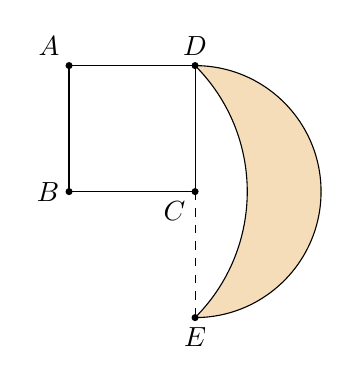
\begin{tikzpicture}[scale=1.6]
\coordinate (C) at (0,0); \coordinate (D) at (0,1); \coordinate (E) at (0,-1);
\coordinate (B) at (-1,0); \coordinate (A) at (-1,1);
\fill[bandamber!30] (0,1) arc (90:-90:1) arc (-45:45:1.4142);
\draw (0,1) arc (90:-90:1);
\draw (0,-1) arc (-45:45:1.4142);
\draw (A)--(D)--(C)--(B)--cycle; \draw[dashed] (C)--(E);
\foreach \p/\q in {A/above left,B/left,C/below left,D/above,E/below}
  \fill (\p) circle (0.8pt) node[\q]{$\p$};
\end{tikzpicture}
\end{center}

\prob{a-means}{Three kinds of middle}{after Q1266, by John Smith}
Take the numbers 4 and 9. Their arithmetic mean is $\tfrac{4+9}{2}$. Their geometric mean
is $\sqrt{4\times9}$. Their harmonic mean is $\tfrac{2\times4\times9}{4+9}$. Work out all
three. Which is largest, and which smallest? Multiply the largest by the smallest. What
do you notice?

\prob{a-shillings}{Half a fortune}{Q1272, by John Epps}
In old money there were 20 shillings in a pound. A sum is $x$ pounds and $y$ shillings.
Half of it is $y$ pounds and $x$ shillings. Find the sum.

\prob{a-squarecube}{Squares and cubes}{Q1291, by John Davey}
Find two whole numbers such that the difference of their squares is a cube and the
difference of their cubes is a square. \textit{Both are less than 12.}

\prob{a-steps}{Three squares in step}{Q1217, by William Saint}
Find three square numbers that are equally spaced, so that the second is as far above
the first as the third is above the second.

\prob{a-equal}{Equal distances}{Q1150, by S.~Jones}
$P$ is a point on the diameter $AD$ of a semicircle, produced beyond $D$. A line from $P$
cuts the semicircle at $C$ and $B$. At $C$ and $B$ lines are drawn at right angles to
$PB$, meeting the diameter at $H$ and $I$. Show that $H$ and $I$ are the same distance
from the centre.

%================ PINK ================
\band{bandpink}{Pink}{ages 14--16}

\prob{p-168}{Plus one}{Q1111, by M.~H.~Murck}
Find two numbers such that each, plus 1, is a square; their sum plus 1 is a square; and
their difference plus 1 is a square.

\prob{p-aces}{All four aces}{Q1120, by Thomas Hopper}
Four people play whist, and each is dealt 13 cards. One offers 100 to 1 that he will have
all four aces. What is the chance that he does? Is his offer a good one for him?

\prob{p-raffle}{The raffle}{after Q1151, by Thomas Hopper}
Four people take turns to throw an eight-sided dice. The first to throw an 8 wins. Find
each person's chance of winning.

\prob{p-arbelos}{The shoemaker's knife}{Q1187, by William Saint}
$ADC$ is a semicircle on the diameter $AC$, and $B$ is any point on $AC$. Semicircles are
drawn inside it on $AB$ and $BC$, and $BD$ is drawn at right angles to $AC$. Show that the
area inside the big semicircle but outside the two small ones equals the area of the
circle with diameter $BD$.
\begin{center}
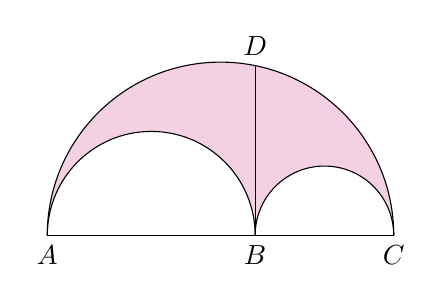
\begin{tikzpicture}[scale=1.1]
\fill[bandpink!25] (-2,0) arc (180:0:2) arc (0:180:0.8) arc (0:180:1.2);
\draw (-2,0) arc (180:0:2); \draw (-2,0) arc (180:0:1.2); \draw (0.4,0) arc (180:0:0.8);
\draw (-2,0)--(2,0); \draw (0.4,0)--(0.4,1.9596);
\node[below] at (-2,0){$A$}; \node[below] at (0.4,0){$B$}; \node[below] at (2,0){$C$};
\node[above] at (0.4,1.96){$D$};
\end{tikzpicture}
\end{center}

\prob{p-cube}{Five squares and a cube}{Q1270, by Thomas Smith}
Find the smallest whole numbers $x$, $y$, $z$ with $5x^2 + y^2 = z^3$.

\prob{p-trees}{Double and double again}{Q1284, by William Wiseman}
Three trees $A$, $B$, $C$ are planted so that the angle at $A$ is twice the angle at $B$,
and the angle at $B$ is twice the angle at $C$. A path of 400\,m runs round all three.
How far apart are they?

\prob{p-construct}{Base, sum and angle}{Q1090, by William Bewley}
Given the base of a triangle, the sum of the other two sides, and the angle between them,
construct the triangle.

\prob{p-reflection}{The tree in the river}{after Q1195, by William Morley}
I stand on the bank of a river that runs west, with my eye 1.5\,m above the water. The top
of a tree directly across the river is reflected in the water 1.8\,m from where I stand. I
walk 18\,m west along the bank, and now the reflection is 2.4\,m from me. How tall is the
tree?

\prob{p-teide}{From the top of Teide}{after Q1210, by John Baines, junior}
A man stands on the summit of Mount Teide, 3,718\,m high, with his eye 1.8\,m above the
rock. He can just see the top of another mountain peeping over the sea horizon. The
straight line from his eye to that top is 430\,km long and just grazes the sea. Taking the
Earth to be a sphere of radius 6,371\,km, how high is the other mountain?

\prob{p-legacy}{Four sons}{Q1209, by Thomas Kirton}
A father leaves \pounds100{,}000 to his four sons, who are 12, 13, 14 and 15 years old.
It is to be divided so that each son, when he comes of age at 21, will have the same
amount, with compound interest at 5\% a year. What does each son receive?

\prob{p-flowerpot}{A litre in a flowerpot}{after Q1135, by the Rev.~William Wright}
A flowerpot is a cone with its tip cut off. Its two ends are 12\,cm and 10\,cm across,
and it holds exactly one litre. How deep is it?

\prob{p-cone}{Five to four}{after Q1166, by W.~Putsey}
A cone holds one litre. Its slant side is to the diameter of its base as 5 is to 4. Find
its height, its slant side and the diameter of its base.

\prob{p-sisters}{Three lovely sisters}{Q1164, by William Moore}
Leybourn prints this one as the Diary did, in verse:
\begin{center}\itshape
Three lovely sisters uncle left\\
To them a piece of gold.\\
Its true dimensions are annex'd,\\
The form of which is told.\\
To part it equally and right,\\
You must cut parallel\\
To its smooth base, and then the height\\
Of each piece truly tell.\\
If this you do 'twill them oblige,\\
For 'tis the old man's wish;\\
And where they live, if there you ride,\\
You'll get from each a kiss.
\end{center}
The gold is the frustum of a paraboloid. Its end diameters are as 2 to 1, and it is
3 inches high. Cut it into three pieces of equal volume. \textit{Hint: a paraboloid
measured from its tip has volume proportional to the square of its height, and its
radius squared is proportional to its height.}

\prob{p-quadrant}{A circle in the corner}{Q1244, by J.~J.~Habershon}
$OBC$ is a quadrant of a circle with centre $O$ and radius $R$. A semicircle is drawn on
the radius $OC$ as diameter. A small circle touches the radius $OB$, the arc $BC$ and the
semicircle. Show that its radius is $R/4$, and that the semicircle has twice its area.

\prob{p-incircles}{Two small circles}{Q1211, by Samuel Titlow}
In a right-angled triangle a perpendicular is dropped from the right angle to the
hypotenuse. Circles are inscribed in the two smaller triangles. Show that their diameters
are in the same ratio as the two shorter sides of the big triangle.

\prob{p-perimeter}{Perimeter and height}{Q1232, by John Ryley}
A right-angled triangle has a perimeter of 24\,cm, and the perpendicular from the right
angle to the hypotenuse is 4.8\,cm. Find its sides. \textit{Hint: if $p$ is the perimeter
and $h$ the perpendicular, the hypotenuse is $p^2/(2p+2h)$. Can you show why?}

\prob{p-fractions}{Sums and differences}{Q1203, by William Saint}
Find two numbers such that their sum, increased or decreased by their difference, gives a
square, and their sum, increased or decreased by the difference of their squares, also
gives a square. \textit{Hint: make the two numbers add up to 1.}

\prob{p-pond}{The fishpond}{after Q1181, by William Burdon}
At the two ends of a diameter of a round pond stand pillars 5\,m and 9\,m high. A ladder
set on the edge of the pond, $30^\circ$ round the edge from the taller pillar, just reaches
the top of either. How wide is the pond?

%================ PURPLE ================
\band{bandpurple}{Purple}{ages 16--17}

\prob{u-thirteen}{Fibonacci's thirteen}{Q1099, by Leonardus Pisanus}
Find a rational number $n$ such that $n^2+13$ and $n^2-13$ are both squares of rational
numbers.

\prob{u-29}{Twenty-nine}{Q1189, by Peter Barlow}
In cribbage you are dealt six cards and keep four; one more card, the starter, is turned
up from the rest of the pack. The best score, 29, needs three fives and the jack of the
fourth suit in your hand, with the fourth five as the starter. What is the chance?

\prob{u-prime}{A prime divides}{Q1205, by Peter Barlow}
The Diary claimed that if $a$ is any prime, then $a$ divides
$1^2+2^2+\dots+\bigl(\tfrac{a-1}2\bigr)^2$, and that the product of those same squares
leaves a remainder of $\pm1$ on division by $a$. Prove what is true, and say where the
claim fails.

\prob{u-view}{The best view}{Q1286, by John Abram}
$A$ and $B$ lie on a straight line through $C$, at 4\,m and 9\,m from $C$. A second line
passes through $C$ at any angle. Where on the second line does $AB$ look largest?

\prob{u-paraboloid}{The paraboloid in the cone}{Q1100, by T.~Hewitt}
Find the height of the largest paraboloid (standing on the base of a cone, tip upwards)
that fits inside the cone. Compare its volume with the cone's and with the largest
cylinder that fits inside the same cone.

\prob{u-around}{The paraboloid round the ball}{Q1260, by W.~Putsey}
A ball has radius 2. Find the paraboloid of least volume that contains it.

\prob{u-ellipses}{Rectangles in ellipses}{Q1294, by William Burdon}
Inscribe the largest rectangle in an ellipse; in that rectangle the largest ellipse; in
that the largest rectangle; and so on for ever. Show that all the rectangles together
have the same area as the rectangle drawn round the first ellipse.

\prob{u-brothers}{Four brothers}{prize question for 1815, by Llerien}
A rectangle has one side equal to the diameter of a circle and the other equal to half its
circumference. Divide it among four brothers into equal shares, using curved fences that
run from one corner to the opposite one.

\prob{u-incircle}{The largest inscribed circle}{Q1201, by T.~Myers}
A right-angled triangle has a circumscribed circle of radius 20\,m. Its inscribed circle is
as large as possible. Find its area.

\prob{u-isoperimetric}{Fixed angle, fixed perimeter}{Q1214, by D.~T.~Sheridan}
Among all triangles with a given perimeter and a given angle at the vertex, show that the
one with the largest area is isosceles.

\prob{u-centroid}{The cone that stands firmest}{after Q1212, by William Burdon}
A cone holds one litre. The perpendicular from its centre of mass to its slant side is as
long as possible. Find the cone.

\prob{u-block}{The block with the given diagonal}{Q1262, by William Burdon}
A block of marble has square ends. The diagonal of one of its long faces is 5\,m. Find the
length and end of the block when its volume is greatest.

\prob{u-beam}{The beam from the tree}{Q1261, by William Burdon}
A tree is a frustum of a cone 9 feet long, 5 feet across at the thick end and 2 feet at
the thin end. A square beam is to be cut from it, starting at the thick end. How long
should it be, to have the greatest volume?

\prob{u-fence}{The shortest fence}{Q1225, by A.~Nesbit}
A triangular field $ABC$ has $AC = 50$ chains, angle $B = 100^\circ17'$, and $AB : BC =
7 : 6$. A straight fence from $AB$ to $BC$ is to cut off half the field. Make it as short
as possible.

\prob{u-roller}{The garden roller}{after Q1105, by William Maddocks}
A stone is a prolate spheroid 100\,cm long and 70\,cm across. The mason wants the
largest cylinder whose axis lies along the long axis. How much must he cut off each end?

\prob{u-line}{A line through a point}{Q1104, by Henry Rocktree}
A point lies inside a given angle. Draw a line through it, cutting the two arms at $A$ and
$C$, so that the product of the lengths from the vertex, $BA\cdot BC$, is as small as
possible.

\prob{u-collinear}{Three points in a line}{Q1138, by Peter Phelan}
The inscribed circle of a triangle touches the base at $E$, and $C$ is the vertex.
Show that the midpoint of $CE$, the centre of the circle and the midpoint of the base lie
on one straight line.

\prob{u-gp}{Three differences}{Q1275, by D.~T.~Sheridan}
In a triangle, the base is cut in two by three different points: the foot of the
perpendicular from the vertex, the point where the inscribed circle touches it, and the
foot of the bisector of the vertical angle. Show that the three differences between the
segments are in geometric progression.

\prob{u-quarter}{Quartering a field}{Q1237, by Robert Rogers}
Cut a given quadrilateral into four equal areas by two straight lines at right angles.
(Most of the Diary's solvers bisected the area one way, then again another way. Why is
that not enough?)

\prob{u-locus}{A straight locus}{Q1183, by Metro}
$AB$ is a chord of a circle with centre $C$, and $D$ is its midpoint. From $D$ any line
$DE$ is drawn to the circle. The perpendicular from $C$ to $DE$ meets the tangent at $E$
in $F$. Show that $F$ always lies on one straight line.

%================ ANSWERS ================
\clearpage
\section*{Answers}

\subsection*{\color{bandgreen}Green}
\ans{g1}{Mark the middle of each side and join the three marks. The four triangles are
the same.}
\ans{g2}{Fold in half, then in half again the same way (four strips); fold in half one
way and then the other (four small rectangles); or fold both diagonals (four triangles,
the same size though not all the same shape). The Diary's brothers used curves; see
problem~\ref{u-brothers}.}
\ans{g3}{4 each; then 5 each.}
\ans{g4}{Ann. Everyone has the same chance on any one roll, but Ann rolls first, so she
has a chance before anyone else does.}

\subsection*{\color{bandblue}Blue}
\ans{b1}{13 and 31: $13^2 = 169$ and $31^2 = 961$. The Diary asked for more: the digits of
169 add to $16 = (1+3)^2$, and $1+3 = 4 = (3-1)^2$. Only 13 and 31 pass every test.}
\ans{b2}{$38^2 = 1444$. The Diary's readers also proved that no square ends in four equal
digits, unless they are zeros.}
\ans{b3}{$8^3 - 7^3 = 512 - 343 = 169 = 13^2$.}
\ans{b4}{6 and 10: $6\times6\times10 = 360$. The Diary also asked for the larger times
itself times the smaller to make 360. That has no whole-number answer.}

\subsection*{\color{bandamber}Amber}
\ans{a-ladder}{If the house is $h$\,m high, $1.2^2 + h^2 = 2^2 + (h-0.4)^2$, so $0.8h =
2.72$ and $h = 3.4$\,m. The ladder is $\sqrt{13}\approx3.61$\,m. In the Diary: 34 feet
and $\sqrt{1300}$ feet.}
\ans{a-pillars}{If the foot is $x$\,m from the short pillar, $x^2 + 4 = (6-x)^2 + 9$, so
$x = 3\tfrac5{12}$\,m. The ladder is about 3.96\,m.}
\ans{a-angles}{9 sides. The outside angles are $60^\circ, 55^\circ, 50^\circ,\dots$ and
must add up to $360^\circ$. Nine of them do. So do sixteen, but then the thirteenth inside
angle would be $180^\circ$, which is impossible.}
\ans{a-trench}{$1.5(D^2 - d^2) = 1 \times d^2$, so $d = D\sqrt{3/5} \approx 15.5$\,m.}
\ans{a-pyramid}{The slant edges equal the base side $s$, and the corner is $s/\sqrt2$
from the centre, so $h^2 = s^2/2$ and $s = 140\sqrt2 \approx 198$\,m. The base is
$2h^2 = 39{,}200$\,m$^2$. The Diary's pyramid, 490 feet high, covered about 11 acres.}
\ans{a-lune}{$BD = BE = s\sqrt2$ and angle $DBE$ is a right angle, so the quarter circle
round $B$ has area $\tfrac\pi4\cdot 2s^2 = \tfrac\pi2 s^2$, the same as the semicircle on
$DE$. Take away the part they share, the segment between arc and chord. What is left is
the lune on one side and the triangle $DBE$ on the other. The triangle is half of
$DE \times BC = 2s\cdot s$, which is $s^2$.}
\ans{a-means}{6.5, 6 and about 5.54. The arithmetic mean is largest, the harmonic
smallest, and $6.5 \times 5.54 = 36 = 6^2$: the geometric mean is the geometric mean of the
other two.}
\ans{a-shillings}{\pounds13 6s. It is 266 shillings, and half of it is 133 shillings, or
\pounds6 13s. The Diary's readers noticed the trick works for a sixth as well:
\pounds17 2s is six times \pounds2 17s.}
\ans{a-squarecube}{10 and 6: $100 - 36 = 64 = 4^3$ and $1000 - 216 = 784 = 28^2$.}
\ans{a-steps}{1, 25 and 49, with a step of 24. There are many more.}
\ans{a-equal}{Let $O$ be the centre and draw $OF$ at right angles to the chord $CB$. It
bisects the chord. $CH$, $OF$ and $BI$ are parallel, all at right angles to $PB$, and
parallel lines cut any two lines in the same ratio. Since $CF = FB$, $HO = OI$.}

\subsection*{\color{bandpink}Pink}
\ans{p-168}{168 and 120: $169$, $121$, $289$ and $49$ are all squares. Writing the numbers
as $x^2+2x$ and $x^2-2x$ settles the first two conditions at once.}
\ans{p-aces}{$\tfrac{13}{52}\cdot\tfrac{12}{51}\cdot\tfrac{11}{50}\cdot\tfrac{10}{49} =
\tfrac{11}{4165}$, about 1 in 379. The fair odds are 4154 to 11, nearly 378 to 1, so
offering only 100 to 1 is a bad bet.}
\ans{p-raffle}{Each chance is $\tfrac78$ of the one before, so they are in the ratio
$512 : 448 : 392 : 343$. The first player wins with probability $\tfrac{512}{1695}\approx
0.302$; then $0.264$, $0.231$ and $0.202$.}
\ans{p-arbelos}{Let $AB = 2a$ and $BC = 2b$. The big semicircle minus the two small ones
is $\tfrac\pi2\bigl((a+b)^2 - a^2 - b^2\bigr) = \pi ab$. Since $ADC$ is a right angle,
$BD^2 = AB\cdot BC = 4ab$, and the circle on $BD$ has area $\pi\cdot BD^2/4 = \pi ab$.
Archimedes knew this figure as the \textit{arbelos}, the shoemaker's knife.}
\ans{p-cube}{$z = 6$, with $5\cdot 2^2 + 14^2 = 216 = 6^3$. The Diary's answer was
$x=2$, $y=14$. One reader pointed out $x = y = z = 6$ as well.}
\ans{p-trees}{The angles are $\tfrac{4\pi}7$, $\tfrac{2\pi}7$ and $\tfrac{\pi}7$. The sides
are in the ratio of their sines, so $BC \approx 79.2$\,m, $AC\approx142.8$\,m and
$AB\approx178.0$\,m.}
\ans{p-construct}{On the base $AB$ draw an arc holding half the given angle. From $A$ mark
$AD$ equal to the given sum, with $D$ on that arc. The perpendicular bisector of $BD$ meets
$AD$ at $C$. Then $CB = CD$, so $AC + CB = AD$, and the angle at $C$ is twice the angle at
$D$.}
\ans{p-reflection}{About 15.5\,m. The reflection divides the line from me to the tree in
the ratio of my eye height to the tree height $H$. So both distances are multiplied by
$1 + H/1.5$ to reach the tree, and the two lines to the tree differ by the 18\,m walk
at right angles. This gives $1 + H/1.5 = 18/\sqrt{2.4^2 - 1.8^2} \approx 11.34$. In the
Diary's feet the tree was 51.7\,ft.}
\ans{p-teide}{From a height $h$ the distance to the horizon is about $\sqrt{2Rh}$. From
the summit that is $\sqrt{2\times 6371\times 3.7198}\approx217.7$\,km. The other
212.3\,km belongs to the other mountain, whose height is $212.3^2/(2\times6371)\approx
3.54$\,km.}
\ans{p-legacy}{The shares go up by a factor of 1.05 each: \pounds23{,}201.18,
\pounds24{,}361.24, \pounds25{,}579.30 and \pounds26{,}858.27. The youngest son's share
waits nine years, the eldest's six. Each son has about \pounds35{,}993 at 21.}
\ans{p-flowerpot}{$V = \tfrac{\pi h}{12}(D^2+Dd+d^2)$, so $h = 12000/(364\pi)\approx
10.5$\,cm.}
\ans{p-cone}{With radius $2t$ and slant $5t$, the height is $\sqrt{21}\,t$. Setting
$\tfrac13\pi(2t)^2\sqrt{21}\,t = 1000$ gives $t\approx3.73$. The base is about 14.9\,cm
across, the slant 18.7\,cm and the height 17.1\,cm.}
\ans{p-sisters}{The radius squared grows with the height, so diameters of 2 to 1 mean
heights of 4 and 1 from the tip. The frustum is then $16-1 = 15$ units of volume, 5 for
each sister. The cuts come where the volume from the tip is 6 and 11, at heights
$\sqrt6$ and $\sqrt{11}$. From the top the pieces are 1.449, 0.867 and 0.683 inches
high.}
\ans{p-quadrant}{Put $O$ at the origin, $C = (R,0)$ and $B = (0,R)$, and let the small
circle have centre $(r,y)$. Touching the arc gives $r^2 + y^2 = (R-r)^2$, so $y^2 =
R^2 - 2Rr$. Touching the semicircle gives $(r-\tfrac R2)^2 + y^2 = (\tfrac R2 + r)^2$,
so $y^2 = 2Rr$. Hence $r = R/4$. Then the semicircle is $\tfrac\pi8 R^2$ and the circle
$\tfrac\pi{16}R^2$.}
\ans{p-incircles}{The two small triangles are similar to each other, and their
hypotenuses are the two shorter sides of the big triangle. In similar triangles every
length, the inscribed diameter included, is in the ratio of the hypotenuses.}
\ans{p-perimeter}{6, 8 and 10\,cm. With legs $a, b$ and hypotenuse $c$, $ab = ch$ and
$a^2+b^2 = c^2$, so $(p-c)^2 = c^2 + 2ch$, giving $c = p^2/(2p+2h) = 10$.}
\ans{p-fractions}{With the sum 1, the difference of squares equals the difference, and the
conditions become: $2a$ and $2b$ are squares with $a+b = 1$. Take $2a = \tfrac{49}{25}$
and $2b = \tfrac1{25}$: the numbers $\tfrac{49}{50}$ and $\tfrac1{50}$ work. There are
infinitely many others, and the Diary's readers found several.}
\ans{p-pond}{About 8.04\,m. With diameter $d$, the ladder's foot is $d\sin15^\circ$ from
the tall pillar and $d\cos15^\circ$ from the short one. So $d^2(\cos^2 15^\circ -
\sin^2 15^\circ) = 81 - 25$, that is $d^2\cos30^\circ = 56$.}

\subsection*{\color{bandpurple}Purple}
\ans{u-thirteen}{$n = \tfrac{106921}{19380}$. Then $n^2 + 13 = \bigl(\tfrac{127729}{19380}
\bigr)^2$ and $n^2 - 13 = \bigl(\tfrac{80929}{19380}\bigr)^2$. Numbers like 13, for
which such an $n$ exists, are now called congruent numbers: they are the areas of
right-angled triangles with rational sides. The Diary's proposer noted the problem in
Luca Pacioli's \textit{Summa} of 1494.}
\ans{u-29}{1 in 216{,}580. The six cards must include the four named cards and two
others that are not the last five: $4\binom{47}{2}$ hands out of $\binom{52}{6}$. The
starter must then be that five, one card among the 46 you have not seen.}
\ans{u-prime}{$\sum_{k=1}^{m}k^2 = \tfrac{m(m+1)(2m+1)}6$ with $m = \tfrac{a-1}2$ gives
$\tfrac{a(a^2-1)}{24}$. For a prime $a>3$, $a^2-1$ is divisible by 24, so $a$ divides the
sum. For $a = 3$ the sum is 1, and the claim fails. For the product: pair each $k$ with
$a-k$. Wilson's theorem, $(a-1)!\equiv-1$, becomes
$\bigl((\tfrac{a-1}2)!\bigr)^2 \equiv (-1)^{(a+1)/2} \pmod a$.}
\ans{u-view}{6\,m from $C$. The best point $D$ is where a circle through $A$ and $B$
touches the second line. Any other point lies outside that circle and sees $AB$ under a
smaller angle. By the tangent--secant theorem $CD^2 = CA\cdot CB = 36$.}
\ans{u-paraboloid}{In a cone of height 1 and base radius 1, a paraboloid with its tip at
height $h$ can be at most as wide as the cone allows. Its volume is greatest when $h =
\tfrac23$. It is then $\tfrac89$ of the cone. That is twice the largest cylinder, which is
$\tfrac49$ of the cone.}
\ans{u-around}{Height $\tfrac{16}3$ and base diameter $\tfrac{16}3$, both equal. The
volume is $\tfrac{512\pi}{27}\approx59.57$. The ball is exactly $\tfrac9{16}$ of it.}
\ans{u-ellipses}{In an ellipse with semi-axes $a, b$ the largest rectangle has sides
$a\sqrt2$ and $b\sqrt2$, area $2ab$. The largest ellipse in that rectangle has semi-axes
$a/\sqrt2$ and $b/\sqrt2$. Each round halves the area, so the rectangles total $2ab(1 +
\tfrac12 + \tfrac14 + \cdots) = 4ab$. That is the area of the rectangle round the first
ellipse, and indeed of every parallelogram whose sides touch it at the ends of two
conjugate diameters.}
\ans{u-brothers}{A half-arch of a cycloid drawn by a circle of diameter $d$ spans exactly
$\tfrac{\pi d}2$ by $d$: it fits the rectangle corner to corner. It cuts off a quarter of
the rectangle. Draw two such arches between the same pair of opposite corners, one bulging
each way. The middle strip that is left is half the rectangle. Draw its diagonal as two
smaller half-arches meeting at the centre, one on each side, and it is halved. As a bonus,
each fence is $2d$ long.}
\ans{u-incircle}{The hypotenuse is the diameter, 40\,m, and the inscribed radius is
$\tfrac12(a + b - 40)$. With $a^2+b^2$ fixed, $a+b$ is largest when $a = b$. The area is
then $40^2/4 = 400$\,m$^2$.}
\ans{u-isoperimetric}{The excircle opposite the vertex touches both arms at a distance
equal to the half-perimeter $s$, so it is fixed. Every triangle in the family has its base
tangent to it. The area is $rs$, so the inscribed radius must be largest. That happens
when the base is at its nearest to the vertex, at right angles to the bisector of the
angle: the isosceles triangle.}
\ans{u-centroid}{The centre of mass is a quarter of the way up. Its distance from the
slant side is $\tfrac34 h\cdot r/\sqrt{h^2+r^2}$. With $\tfrac13\pi r^2h$ fixed, this is
greatest when $h^2 = 2r^2$. For one litre, $h\approx12.41$\,cm and the base is about
17.55\,cm across.}
\ans{u-block}{If the length is $L$ and the end is $s$ square, $L^2+s^2 = 25$ and $Ls^2$
must be greatest. So $s^2 = 2L^2$, $L = 5/\sqrt3\approx2.89$\,m and $s = 5\sqrt{2/3}
\approx4.08$\,m.}
\ans{u-beam}{At $x$ feet from the thick end the tree is $D = 5 - \tfrac x3$ feet across.
The beam has volume $\tfrac12 D^2x$, greatest when $D = \tfrac23x$, that is at $x = 5$.
The beam is 5 feet long, cut where the tree is $3\tfrac13$ feet across. Its square end
has side $3\tfrac13/\sqrt2\approx2.36$ feet.}
\ans{u-fence}{The sides come out as $AB = 35$ and $BC = 30$ chains exactly. For a given
area, the fence is shortest when it cuts off an isosceles triangle at $B$. So $BD = BE =
\sqrt{\tfrac12\cdot35\cdot30} = \sqrt{525}\approx22.91$ chains, and the fence is about
35.18 chains.}
\ans{u-roller}{The largest cylinder has length $100/\sqrt3\approx57.7$\,cm, so cut
$21.1$\,cm off each end. One solver, Olinthus Gregory, added that a cylinder with its axis
across the stone, along the 70\,cm axis, is larger still, in the ratio 10 to 7.}
\ans{u-line}{The product $BA\cdot BC$ is proportional to the area of triangle $ABC$,
since the angle at $B$ is fixed. The area is smallest when the given point is the
midpoint of $AC$. Draw it by marking the same distance on the far side of the point.}
\ans{u-collinear}{Let $E'$ be the point of the circle opposite $E$. The line $CE'$ meets
the base at $F$, where the excircle touches it, and $AE = BF$, so the midpoint $M$ of the
base is also the midpoint of $EF$. The centre $O$ is the midpoint of $EE'$. So $MO$ is
parallel to $FE'C$, and a line through the midpoint of $EF$ parallel to $FC$ bisects
$EC$.}
\ans{u-gp}{With sides $a$ and $c$ at the vertex and base $b$, the three differences are
$\tfrac{a^2-c^2}{b}$, $a-c$ and $\tfrac{(a-c)b}{a+c}$. Each is $\tfrac{b}{a+c}$ times the
one before.}
\ans{u-quarter}{If one line halves the field and another halves it too, the four pieces
$p, q, r, s$ satisfy $p+q = r+s$ and $p+r = q+s$. That gives $p = s$ and $q = r$, but not
$p = q$. Four equal parts need a third condition, and the lines must also be at right
angles. Leybourn's editor showed that the problem leads to an equation of high degree,
and cannot in general be done with ruler and compasses.}
\ans{u-locus}{Let $CF$ meet $DE$ at $H$, at right angles. Triangle $CEF$ has a right
angle at $E$, so $CH\cdot CF = CE^2 = r^2$. The circle on diameter $DF$ passes through
$H$; drop $FK$ at right angles to $CD$ produced, and $K$ is on it too. So $CD\cdot CK =
CH\cdot CF = r^2$. $CK$ is fixed, and $F$ lies on the line through $K$ parallel to $AB$.}

\begin{diarynote}{When the Diary was wrong}
\textbf{Problem~\ref{u-prime}.} The claim was printed for ``any prime number'', and every
solver proved it for every prime. It is false for 3.

\textbf{Problem~\ref{u-thirteen}.} This was the second time of asking. The question had
already appeared in the Diary for 1800, and the answers printed then did not make $n$
rational. The proposer, signing as Leonardo of Pisa, set it again.

\textbf{Problem~\ref{u-29}.} The Diary reached 1 in 216{,}580, which is right. Its
reasoning allowed the last five into the hand, then made the starter one of 48 cards
rather than 46. The two slips cancel exactly.

\textbf{Problem~\ref{u-quarter}.} Several solvers claimed to quarter the field by
bisecting it twice. The editor printed their names and explained why this does not work.

\textbf{Problem~\ref{p-trees}.} The solvers disagreed in the first decimal place. One took
the sine of $102^\circ51'$ as 0.97438, not 0.97493; another slipped in the arithmetic.

\textbf{Problem~\ref{u-beam}.} The printed solution gives $3\tfrac13$ feet as ``each side of
the ends of the beam''. That is the tree's diameter at the cut, the diagonal of the
beam's square end. The side is about 2.36 feet.

\textbf{Problem~\ref{p-cube}.} It was printed twice. The same question appears again as
Q1285, with an editor's note that it was ``by mistake, inserted over again''.
\end{diarynote}

\end{document}
